\documentclass[letter, 10pt]{article}
\usepackage[utf8]{inputenc}
\usepackage[spanish]{babel}
\usepackage{amsfonts}
\usepackage{amsmath}
\usepackage[dvips]{graphicx}
\usepackage{subfigure}
\usepackage{url}
\usepackage{hyperref}
\usepackage{color}
\usepackage[top=3cm,bottom=3cm,left=3.5cm,right=3.5cm,footskip=1.5cm,headheight=1.5cm,headsep=.5cm,textheight=3cm]{geometry}
\usepackage{alltt}

\definecolor{red}{rgb}{1,0,0}
\definecolor{green}{rgb}{0,1,0}
\definecolor{blue}{rgb}{0,0,1}
\newcommand{\blue}{\textcolor{blue}}
\newcommand{\red}{\textcolor{red}}
\newcommand{\green}{\textcolor{green}}

\begin{document}

\title{
\includegraphics[width=0.9\textwidth]{img/logos.pdf}\\\vspace{1cm}
First Python Programming Course Report}
\author{Computer Systems Research Group (CSRG)}
\date{\today}

\maketitle

\section{Course format}

\subsection{Description}

The objective of the course for the students
is to be able to program in Python~\footnote{\url{http://python.org}}
in order to use effectively the object-oriented interface of ALMA devices.

The target audience is: electronic engineers, mechanical engineers, telescope operators. 

The duration of the course is \emph{4 months}, and the program is divided into \emph{two-week periods},
so that each period covers all the shift rotations of the observatory.

The program details are in the Appendix I~\ref{cap:program}.

The expected student dedication is \emph{8 hours per biweekly period},
so the total expected student dedication for the course is \emph{64 hours}.

The activities for each biweekly period are:
\begin{itemize}
    \item the study of four focused topics, each with simple exercises;
          each topic is expected to be learn and understood in 1 and a half hour.
    \item an assignment that integrates the four focused topics;
          the expected dedication is 2 hours.
\end{itemize}

The students are expected to hand in the solved exercises and assignments
during the course of the corresponding biweekly period,
but late submissions will be accepted within the following period.

\subsection{Evaluation}

The evaluation consists in the grading of each biweekly assignment with
a grade between \emph{0 and 100}.

The final grade is the average of all the assignment grades,
being the minimal passing final grade a \emph{60}. 

Only the \emph{assignments} are the evaluated instances,
the exercises are only to training the student knowledge. 

Each day of delay \emph{reduce 10 points} of the assignment grade. 

The assignment time limit:
\begin{itemize}
    \item Two weeks once is published.
    \item You can obtain an extra week if you have some problem.
\end{itemize}

\subsection{Bibliography}

The used and recommended course bibliography is the following:

\begin{itemize}
    \item Allen B. Downey. Python for Software Design: How to Think Like a Computer Scientist. Green Tea Press, 2008.
    \item Course handout.
    \item Python 2.7 official documentation~\footnote{\url{http://docs.python.org}}.
\end{itemize}

\subsection{Course material}

The course material was prepared using the Python Sphinx module~\footnote{\url{http://sphinx.pocoo.org/}},
and is available in the following URL:

\begin{itemize}
    \item \url{http://csrg.cl/~cmaureir/python-course/}
\end{itemize}

\subsection{Course platform}

The used course platform is Claroline~\footnote{\url{http://www.claroline.net/}},
and is available in the following URL:

\begin{itemize}
    \item \url{http://claroline.aiv.alma.cl/claroline/course/index.php?cid=PPC01}
\end{itemize}

This platform provide several functionality to the course,
for example:
\begin{itemize}
    \item Forums: Used to discuss some lectures and assignments issues.
    \item Announcements: Sending message to all the students.
    \item Assignments: Providing a space to upload assignments files, give feedback and add grades.
\end{itemize}

\subsection{Contact}

The contact information given to the students
is the following:

\begin{itemize}
    \item Email: \url{cmaureir@csrg.cl}
    \item Yahoo Messenger: \url{maureira.cristian}
\end{itemize}

Several students prefer to send to the course instructor personal emails,
instead of write in the course forums.

\section{Conclusion}

\subsection{General}

After finish the first python programming course,
there are some issues, which are important to comment:

\begin{itemize}
    \item Considering that in ALMA the common language is English,
          and also, that the course was asked to be in the same language,
          a lot of students was very uncomfortable with this  issue,
          so in the middle of the course, Spanish forums was created,
          to discuss the students doubts, and also the possibility to
          write doubts emails in Spanish too.

          Maybe, thinking in future courses, will be better for those
          students to provide an English-Spanish course.

    \item Most of the students ask for more time in each period,
          and considering the two weeks for reading and write the assignment,
          was a very strange situation, because was a lot of time,
          but when the students clarify this situation,
          they says that does not have enough time, because they do not
          have assigned time for the course, and most of them used their
          free time to read the lectures and write the assignment.

          Is very unfair for the students because if their
          work responsible give the possibility to take the course,
          will be a good idea to assign a couple of hours per week,
          to dedicate only to the course.

    \item Before the course creation, the people who discuss the course,
          define the target audience which was:
          \begin{itemize}
              \item electronic engineers,
              \item mechanical engineers,
              \item telescope operators.
          \end{itemize}

          But this information is not enough, why?
          because there are people with different academic degrees,
          which implies that some people never programmed before,
          and other students have a lot of programming experience.

          The course was wrote thinking in a medium level,
          but some students says that the course is not basic,
          and they looking for a programming introduction,
          in the other side, students says that the course is
          very basic and they was looking for a more advance course.

          Will be great if in future courses, all the students
          has the same level, i.e. have or have not programming experience.

    \item Every students have some questions in different lectures,
          but there are very shy students, that does not ask the instructor
          their doubts, and prefer to ask other people, which is not
          a negative issue, but will be good to know what are the weak points
          of the lectures, like a feedback, so will be very positive to
          ask to the students that in front of any doubt, send an email
          to the instructor or post in the course forums.

          Following the same idea, given the course characteristics
          there are a miscommunication between some students and the instructor,
          which cause the total lost of communication in for example
          the justification for does not send some assignments.
          As you can see in the Appendix II~\ref{cap:grades},
          some students does not send their assignments,
          and does not answer to the course instructor,
          giving the reason of this absence.

          Could be very positive to any future course,
          to provide access to the students work responsible,
          which will be very effective at the time to ask
          and resolve this kind of problems,
          or maybe an special external person,
          which can access to this students any time..
\end{itemize}

\subsection{Survey}

The survey questions can be found in the Appendix III\ref{cap:survey},
and the answers in the Appendix IV\ref{cap:answers}.

The survey was answered only by 6 students,
and was conducted in the middle of the course. 

Taking into account the student opinion,
there was a very good opportunity to learn a new programming language,
because in some work related task they know the importance of Python and scripting,
and that is very consistent with their work.

The course was considers as a medium difficulty course,
which is a very good opinion because at the beginning of the course,
the students occupation was unknown, so there are people with
different knowledge, and academic degrees.

The assignments was frequently consistent with the lectures exercises
and content, and the students use internet and the course material
to solve any exercise and assignment.

When the students have doubts, the instructor answers was quicker,
and the students show very satisfied with the answer.

Related to the spend time in the course,
the students take more than two hours to read and understand the lectures
each week, and solve the assignments using between 3 to 5 hours.

Also, the students are very enthusiastic to receive more courses,
specially an 'Advance Python Course' and a 'Java Course', etc.

The weak course things that the students wants to improve are:
\begin{itemize}
    \item A on-campus class per week.
    \item Use another online platform instead of claroline (i.e. moodle).
    \item More relation between the lectures exercises and the weekly assignments.
    \item Improve the English redaction.
\end{itemize}


Finally, the general course thoughts are:

\begin{itemize}
    \item The course was very good, but they does not have enough time.
    \item Was a motivational course.
    \item They are satisfied with the course.
    \item Some people never programmed before, and they think that was a very good opportunity to learn.
    \item The course was useful for their work.
\end{itemize}

\newpage
\section{Appendix}
\subsection{Appendix I - Program}
\label{cap:program}
\begin{footnotesize}
\begin{tabular}{p{0.5\textwidth}p{0.5\textwidth}}

\begin{itemize}
    \item First week
    \begin{itemize}
        \item Lecture 1 - Program development
        \item Lecture 2 - Algorithm elements
        \item Lecture 3 - Data types
        \item Lecture 4 - Data types
        \item Assignment 1
    \end{itemize}
    \item Second week
    \begin{itemize}
        \item Lecture 5 - Input and output
        \item Lecture 6 - Control statements
        \item Lecture 7 - Loops
        \item Lecture 8 - Functions
        \item Assignment 2
    \end{itemize}
    \item Third week
    \begin{itemize}
        \item Lecture 9 - Lists
        \item Lecture 10 - Sets
        \item Lecture 11 - Dictionaries
        \item Lecture 12 - Tuples
        \item Assignment 3
    \end{itemize}
    \item Fourth week
    \begin{itemize}
        \item Lecture13 - Modules
        \item Lecture 14 - Modules creation
        \item Lecture 15 - Use of objects and Files
        \item Lecture 16 - Errors and exceptions
        \item Assignment 4
    \end{itemize}
\end{itemize}
&
\begin{itemize}
    \item Fifth week
    \begin{itemize}
        \item Lecture 17 - Advanced topics on functions
        \item Lecture 18 - Higher-order functions
        \item Lecture 19 - Iterators
        \item Lecture 20 - Coding good practices
        \item Assignment 5
    \end{itemize}
    \item Sixth week
    \begin{itemize}
        \item Lecture 21 - Class creation
        \item Lecture 22 - More on class creation
        \item Lecture 23 - Inheritance
        \item Lecture 24 - Design good practices
        \item Assignment 6
    \end{itemize}
    \item Seventh week
    \begin{itemize}
        \item Lecture 25 - NumPy arrays (part I)
        \item Lecture 26 - NumPy arrays (part II)
        \item Lecture 27 - NumPy arrays (part III)
        \item Lecture 28 - Interactive matplotlib plots
        \item Assignment 7
    \end{itemize}
    \item Eighth week
    \begin{itemize}
        \item Lecture 29 - IPython
        \item Lecture 30 - Control Command Language (CCL) Introduction
        \item Lecture 31 - Graphical Interfaces
        \item Lecture 32 - An extra bite of Python
        \item Assignment 8
    \end{itemize}
\end{itemize}
\\
\end{tabular}
\end{footnotesize}

\newpage
\subsection{Appendix II - Grades}
\label{cap:grades}
\vspace{1cm}

\begin{center}
    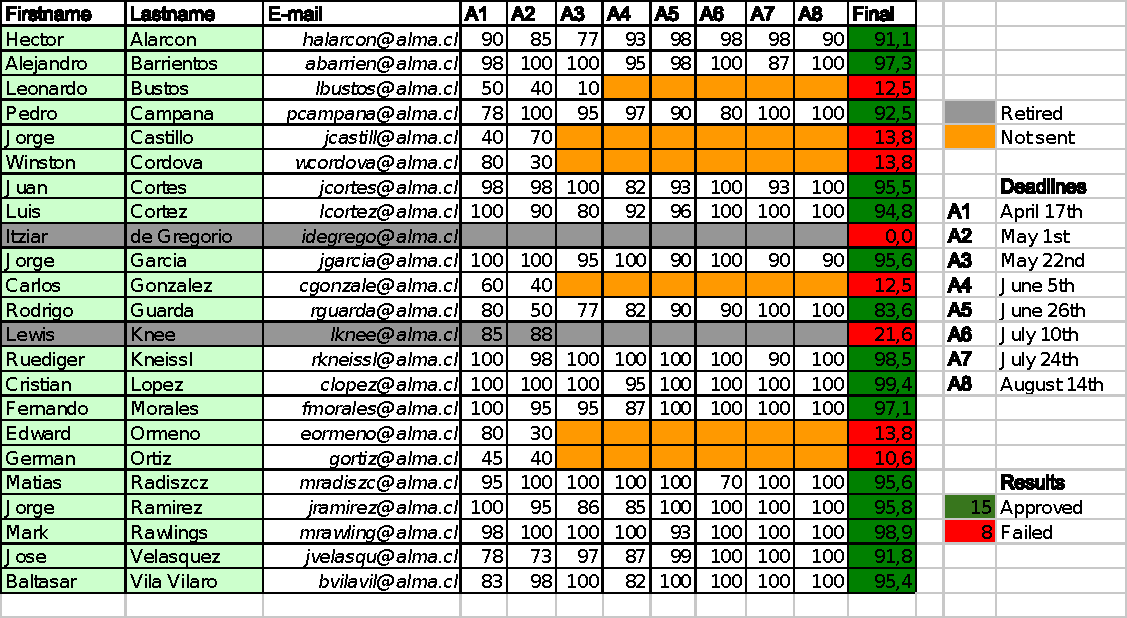
\includegraphics[width=0.99\textwidth]{img/python-course-grades.pdf}
\end{center}

\newpage
\subsection{Appendix III - Survey questions}
\label{cap:survey}
\begin{footnotesize}
\begin{enumerate}
    \item Do you like to learn new programming languages? Why?
    \item Which of the following alternatives do you consider better describe the level of difficulty of the course?
    \begin{enumerate}
        \item Low difficulty
        \item Medium Difficulty
        \item High Difficulty
    \end{enumerate}
    \item Is the level of the course consistent with what you have to do in your work? Why?
    \item Are the evaluations in accordance with the content taught in the course?
    \begin{enumerate}
        \item Always
        \item Frequently
        \item Sometimes
        \item Rarely
        \item Never
    \end{enumerate}
    \item  What did you resort to solve the tasks and / or assignments?
    \begin{enumerate}
        \item Internet
        \item Books
        \item Assistant and/or Teachers
        \item Only Classes
    \end{enumerate}
    \item How long have you had to wait for the teacher responses about your doubts (E-mail or Another way) to allow you to continue your assignments?
          (If you haven’t asked anything please go to question 8)
    \begin{enumerate}
        \item Less than one day
        \item One day to less than three days
        \item Three days or more
    \end{enumerate}
    \item What is your level of satisfaction with the replies to your questions?
    \begin{enumerate}
        \item Very Unsatisfied
        \item Somewhat Unsatisfied
        \item Neutral
        \item Somewhat Satisfied
        \item Very Satisfied
    \end{enumerate}
    \item How much time do you spend reading and reviewing the course’s content? (hours per week)
    \begin{enumerate}
        \item Less than 1 hour
        \item 1 hour to less than 2 hours
        \item 2 hours or more
        \item 1 day or more
    \end{enumerate}
    \item How much time do you spend doing exercises and assignments?
    \begin{enumerate}
        \item Less than 3 hours
        \item 3 hours to less than 5 hours
        \item 5 hours or more
        \item 1 day or more
    \end{enumerate}
    \item Select all the topics that you think would reflect an improvement in your work activities if you were to learn them.
    \begin{enumerate}
        \item Linux Basic Course
        \item PHP
        \item BASH
        \item Java
        \item Advance Python Course
    \end{enumerate}
    \item What aspects would you improve for future versions of the course?
    \item What is your general opinion about the course?
\end{enumerate}
\end{footnotesize}

\subsection{Appendix IV - Survey results}
\label{cap:answers}

\begin{itemize}
    \item Question 1:\\
     \begin{itemize}
        \item Yes, have been very fun to have to think a lot to solve the problems gave every second week
        \item I like to learn Programming language due to is a powerful tool that can help in every aspect and engineering discipline .
        \item Yes. Each of the new programming paradigms works best for some of the problems I need to tackle. So, the more languages I know, the better I can tailor my programming to a given problem.
        \item Yes.
        \item Yes, because is helping with my duties. Specially creating procedures to do routinary tasks which are facilitating the way how to monitoring complex systems.
        \item Very much. It's generally a useful skill to have, and particularly so in the case of Python for ALMA. Most of the programming languages with which I was most familiar are rather old-fashioned at this point, and finding the time to learn a whole new language entirely on my own outside of work is difficult.
     \end{itemize}

    \item Question 2:
        \begin{center}
            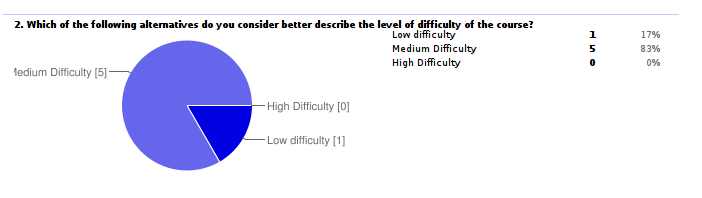
\includegraphics[width=0.9\textwidth]{img/survey_2.png}
        \end{center}

    \item Question 3
    
    \begin{itemize}
        \item well, I still don't know but I think that is consistent with the time that I have and I'll apply the course in my job for sure
        \item It is consistent due to in my job I work with Python scripting and if I want to investigate in what does that scripts do  I have to learn python
        \item Not completely. I expect I will need a more advanced course later to get deeper into the OOP model, and also would like to learn more on the use of Python for IPC.
        \item Yes.
        \item So far so good, but still we need to see more than 50\% of the lectures.
        \item Yes, I think so. Currently have to edit and/or create Python-based scripts, so it seems to be a reasonably good match.
    \end{itemize}
    

    \item Question 4
        \begin{center}
            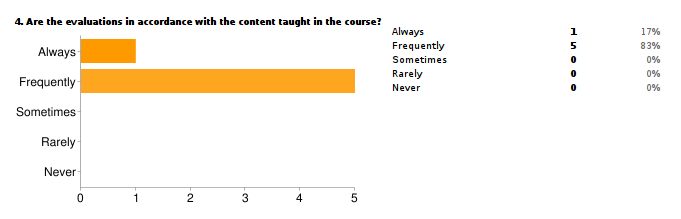
\includegraphics[width=0.9\textwidth]{img/survey_4.png}
        \end{center}
        

    \item Question 5
        \begin{center}
            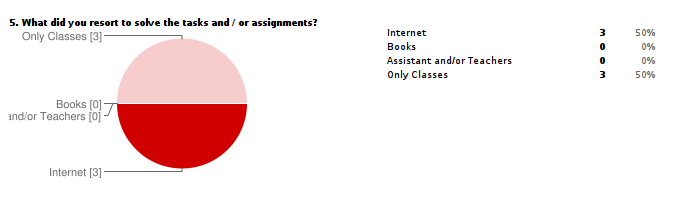
\includegraphics[width=0.9\textwidth]{img/survey_5.png}
        \end{center}

    \item Question 6
        
        \begin{center}
            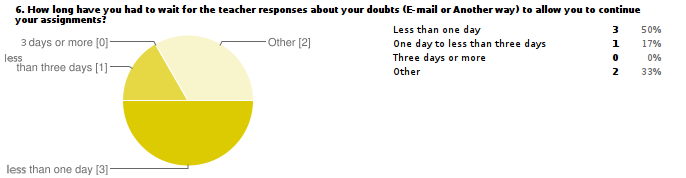
\includegraphics[width=0.9\textwidth]{img/survey_6.png}
        \end{center}

    \item Question 7
        
        \begin{center}
            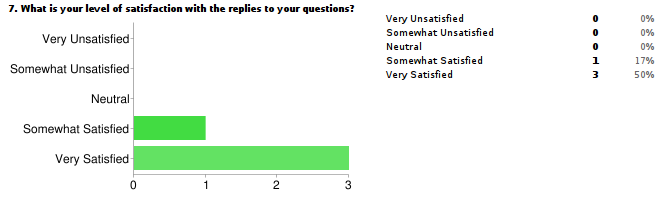
\includegraphics[width=0.9\textwidth]{img/survey_7.png}
        \end{center}

    \item Question 8
        
        \begin{center}
            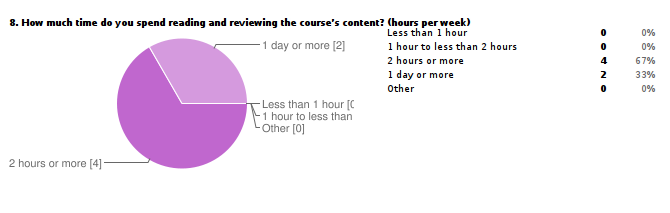
\includegraphics[width=0.9\textwidth]{img/survey_8.png}
        \end{center}
        

    \item Question 9

        \begin{center}
            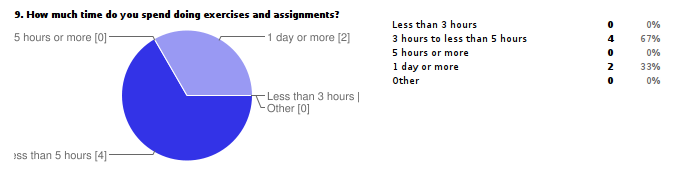
\includegraphics[width=0.9\textwidth]{img/survey_9.png}
        \end{center}
        

    \item Question 10

        \begin{center}
            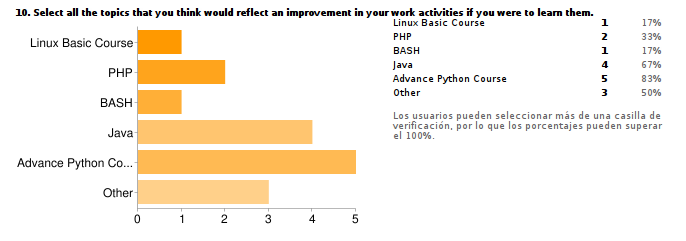
\includegraphics[width=0.9\textwidth]{img/survey_10.png}
        \end{center}

    \item Question 11

    \begin{itemize}
        \item At least one hour of formal classes by week
        \item Some Teachers classes stead of online course
        \item "English must be improved in some of the contents of the lessons.
        \item If possible, it would be nice to get some training into the GUI capabilities, plotting and mathematical Python"
        \item I would use another web platform, like moodle. 
        \item "Probably some fine tuning between the exercises and assignment are necessary. Also a material review is required to remove some Spanish expressions on the English context and some errors in the assignment, as well. But in general are only minor details, and nothing about the content itself."
        \item Generally pretty satisfied as it is. A bit of proof-reading of the English might occasionally help. Including a link to something like: http://www.texify.com might help to make the embedded LaTeX equations easier to work with. 
    \end{itemize}


    \item Question 12

    \begin{itemize}
        \item I have been very interesting and motivating
        \item It is a good course, sometimes I don't have much time to spent on the course (due to my work and rest week off) and sometimes there is not enough time to do the assignments (shifts doesn't concur with the course). Also it would be better to have a teacher's class stead of an online course. Anyway the course is up to my expectations.
        \item I am satisfied on how it is going so far (still half way)
        \item Very good.
        \item The level of the course is adequate to my expectation, I don't have previous experience with programming courses, however often I need to write simple scripts. With courses like this are helping to have more organized and structured code.
        \item Very positive. It's a lot of work, and I find myself short on time/late for it sometimes. However, the timescales involved at least motivate me to try to keep up to date with it, and not set it off to one side in favour of other work very much. I feel that I've learned a lot already.
    \end{itemize}

\end{itemize}
\end{document} 
